\let\negmedspace\undefined
\let\negthickspace\undefined
\documentclass[journal]{IEEEtran}
\usepackage[a5paper, margin=10mm, onecolumn]{geometry}
%\usepackage{lmodern} % Ensure lmodern is loaded for pdflatex
\usepackage{tfrupee} % Include tfrupee package

\setlength{\headheight}{1cm} % Set the height of the header box
\setlength{\headsep}{0mm}     % Set the distance between the header box and the top of the text

\usepackage{gvv-book}
\usepackage{gvv}
\usepackage{cite}
\usepackage{amsmath,amssymb,amsfonts,amsthm}
\usepackage{algorithmic}
\usepackage{graphicx}
\usepackage{textcomp}
\usepackage{xcolor}
\usepackage{txfonts}
\usepackage{listings}
\usepackage{enumitem}
\usepackage{mathtools}
\usepackage{gensymb}
\usepackage{comment}
\usepackage[breaklinks=true]{hyperref}
\usepackage{tkz-euclide} 
\usepackage{listings}
% \usepackage{gvv}                                        
\def\inputGnumericTable{}                                 
\usepackage[latin1]{inputenc}                                
\usepackage{color}                                            
\usepackage{array}                                            
\usepackage{longtable}                                       
\usepackage{calc}                                             
\usepackage{multirow}                                         
\usepackage{hhline}                                           
\usepackage{ifthen}                                           
\usepackage{lscape}

\newcommand{\nCr}[2]{\,^{#1}C_{#2}}

\begin{document}

\bibliographystyle{IEEEtran}
\vspace{3cm}

\title{11.16.3.8.5}
\author{EE24BTECH11012 - Bhavanisankar G S}
% \maketitle
% \newpage
% \bigskip
{\let\newpage\relax\maketitle}

\renewcommand{\thefigure}{\theenumi}
\renewcommand{\thetable}{\theenumi}
\setlength{\intextsep}{10pt} % Space between text and floats


\numberwithin{equation}{enumi}
\numberwithin{figure}{enumi}
\renewcommand{\thetable}{\theenumi}

\textbf{QUESTION} : \\
Three coins are tossed once. Find the probability of getting no head.\\
\textbf{SOLUTION} : \\

 \begin{table}[h!]
    \centering
    \begin{tabular}{|c|c|}
        \hline
        \textbf{One end of Jumper Wire}  & \textbf{Another end of Jumper Wire} \\
        \hline
          Digital pin 0 & Push button 16 \\
          Digital pin 1 & Push button 17 \\
          Digital pin 2 & LCD pin 4 \\
          Digital pin 3 & LCD pin 6 \\
          Digital pin 4 & LCD pin 11 \\
          Digital pin 5 & LCD pin 12 \\
          Digital pin 6 & LCD pin 13 \\
          Digital pin 7 & LCD pin 14 \\
          Digital pin 8 & Push button 18 \\
          Digital pin 9 & Push button 19 \\
          Digital pin 10 & Push button 20 \\
          Digital pin 11 & Push button 21 \\
          Digital pin 12 & Push button 22 \\
          Digital pin 13 & Push button 23 \\
          Analog pin A1 & Push button 15 \\
          Analog pin A2 & Push button 14 \\
          Analog pin A3 & Push button 13 \\
          Analog pin A4 & Push button 12 \\
          Analog pin A5 & Push button 11 \\
          Analog pin A0 & Push buttons 1-10 (digit buttons)\\
          LCD pin 1 & Ground \\
          LCD pin 2 & 5V \\
          LCD pin 15 & 5V via 1k $\Omega$ resistor \\
          LCD pin 16 & Ground \\
          LCD pin 3 & Ground via 1.5 k $\Omega$ resistor \\
          LCD pin 5 & Ground \\
          LCD pin 5 & All push buttons \\
          
        \hline
    \end{tabular}
\end{table}

Let us assume the random variable to be the sum of three Bernoulli Random Variables.
\begin{align}
	\vec{X} &= \vec{X_{1}} + \vec{X_{2}} + \vec{X_{3}} \\
	\vec{X_{i}} &= 
	\begin{cases}
		1 & , \text{ Outcome - head } \\
		0 & , \text{ Outcome - tail }
	\end{cases} \\
	\implies p_{X_{i}} (k) &= 
	\begin{cases}
		1 - p & , k = 0 \\
		p & , k = 1
	\end{cases}
\end{align}
Considering all the outcomes as equally likely, we have
\begin{align}
	p &= \frac{1}{2} \label{eq:p}
\end{align}
For the given question, let $\vec{X}$ denote the number of heads. The sample space corresponding to the given scenario is tabulated below. \\
 \begin{table}[h!]
    \centering
    \begin{tabular}{|c|c|}
        \hline
        \textbf{Button number}  & \textbf{Function} \\
        \hline
           1 - 10 & Digits 0 - 9 \\
           11 & Clear \\
           12 & $\ln{(x)}$ and $\log{(x)}$ \\
           13 & Right Parenthesis \\
           14 & $\sin{(x)}$, $\cos{(x)}$, and $\tan{(x)}$ \\
           15 & $e$ and $\pi$ \\
           16 & Backspace \\
           17 & Decimal Point \\
           18 & Equal To \\
           19 & Left Parenthesis \\
           20 & Division (/)\\
           21 & Multiplications (*)\\
           22 & Subtraction(-) \\
           23 & Addition (+) \\
        \hline
    \end{tabular}
\end{table}

By the properties of Z-transform of \textbf{Probability Mass Function}, we have
\begin{align}
	M_{\vec{X}} (z) &= M_{\vec{X_{1}}} (z) M_{\vec{X_{2}}} (z) M_{\vec{X_{3}}} (z) \\
	M_{\vec{X_{1}}} &= \sum_{n = - \infty}^{\infty} p_{\vec{X_{1}}} (n) z^{-n} = (1 - p) + \brak{p}z^{-1} \\
	M_{\vec{X_{2}}} &= \sum_{n = - \infty}^{\infty} p_{\vec{X_{2}}} (n) z^{-n} = (1 - p) + \brak{p}z^{-1} \\
	M_{\vec{X_{3}}} &= \sum_{n = - \infty}^{\infty} p_{\vec{X_{3}}} (n) z^{-n} = (1 - p) + \brak{p}z^{-1} \\
	M_{\vec{X}} (z) &= \brak{(1 - p) + \brak{p}z^{-1}}^3 \\
	                &= \sum_{k = -\infty}^{\infty} \nCr{3}{k} \brak{1-p}^{3-k} p^{k} z^{-k} \\
	p_{\vec{X}} (k) &= \nCr{3}{k} \brak{1-p}^{3-k} p^{k} \label{eq:pm}
\end{align}
Substituting \eqref{eq:p} in \eqref{eq:pm}, we have
\begin{align}
	p_{\vec{X}} (k) &= \frac{\nCr{3}{k}}{8} \label{eq:pmf}
\end{align}

The PMF is then given by - 
\begin{align}
p_{\vec{X}} (k) &= 
\begin{cases}
	\frac{\nCr{3}{k}}{8} & 0 \leq k \leq 3, k \in \mathbb{W} \\
	0 & otherwise
\end{cases} \\
\implies p_{\vec{X}} (k) &= 
\begin{cases}
	\frac{1}{8} & k = 0 \\
	\frac{3}{8} & k = 1 \\
	\frac{3}{8} & k = 2 \\
	\frac{1}{8} & k = 3 \\
	0 & \text{ otherwise }
\end{cases}
\end{align}

The corresponding \textbf{Cumulative Distribution Function} can then be written as - 
\begin{align}
  F_{X}\brak{k} = \sum_{i = -\infty}^n\comb{3}{i}\brak{\frac{1}{2}}^3 = \begin{cases}
    0 & k < 0\\
    \comb{3}{0}\brak{\frac{1}{2}}^3 = \frac{1}{8} & 0 \le k < 1\\
    \comb{3}{1}\brak{\frac{1}{2}}^3 + \comb{3}{0}\brak{\frac{1}{2}}^3 = \frac{4}{8}& 1 \le k < 2\\
    \comb{3}{2}\brak{\frac{1}{2}}^3 + \comb{3}{1}\brak{\frac{1}{2}}^3 + \comb{3}{0}\brak{\frac{1}{2}}^3 = \frac{7}{8} & 2 \le k < 3\\
    \comb{3}{3}\brak{\frac{1}{2}}^3 + \comb{3}{2}\brak{\frac{1}{2}}^3 + \comb{3}{1}\brak{\frac{1}{2}}^3 + \comb{3}{0}\brak{\frac{1}{2}}^3= 1 & k \geq 3\\
  \end{cases}
\end{align}


\begin{align}
\implies F_{\vec{X}}(k) = Pr(\vec{X} \leq k) =
\begin{cases}
    0 & k < 0 \\
    \frac{1}{8} & 0 \leq k < 1 \\
    \frac{1}{2} & 1 \leq k < 2 \\
    \frac{7}{8} & 2 \leq k < 3 \\
    1 & k \geq 3
\end{cases}
\end{align}
\begin{align}
	F_{\vec{X}} \brak{0} &= P \brak{ \vec{X} <= 0 } \\
	                     &= \frac{1}{8}
\end{align} \\

\textbf{Simulation : } \\
\begin{enumerate}
	\item Generate a random number using the \textbf{rand()} function. 
	\item Restrict the random number to either $0$ or $1$ by using rand() \% 2 operator, and assign it to head ( H ) and tail ( T ).
	\item Count the number of favourable outcomes by iterating for a large number of trials.
	\item Divide it by the total number of trials to get the desired PMF.
	\item CDF can then be simulated by summing the required PMFs.
\end{enumerate}
\begin{figure}[h]
\centering
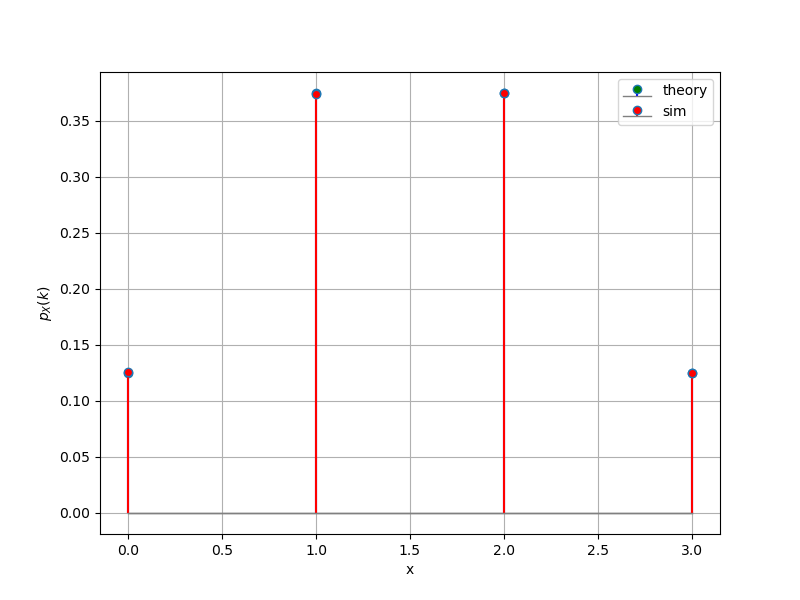
\includegraphics[width=\columnwidth]{figs/pmf.png}
\caption{Probability Mass Funtion}
\label{fig:Plot1} 
\end{figure}

\begin{figure}[h]
\centering
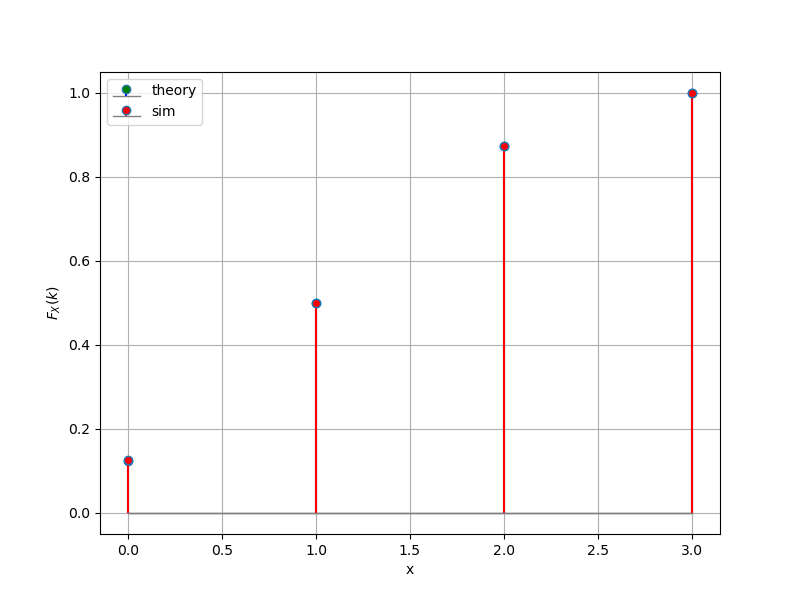
\includegraphics[width=\columnwidth]{figs/cdf.png}
\caption{Cumulative Distribution Function}
\label{fig:Plot1} 
\end{figure}

\end{document}
